\documentclass[a4paper,11pt,twoside,openright]{article}

\usepackage[toc,page]{appendix}
\usepackage{amsmath}
\usepackage{geometry}
\usepackage{graphicx}
\usepackage{subcaption}
\usepackage{multirow}
\usepackage[section]{placeins}
\usepackage{array}
\usepackage[nottoc,numbib]{tocbibind}
%\usepackage{titlesec}

\geometry{margin=1in}
\graphicspath{ {Images/} }

\newcolumntype{?}[1]{!{\vrule width #1}}
\newcommand{\Mod}[1]{\ (\mathrm{mod}\ #1)}

\let\oldsection\section
\def\section{\cleardoublepage\oldsection}

%\setcounter{tocdepth}{4}

%\titleformat{\paragraph}
%{\normalfont\normalsize\bfseries}{\theparagraph}{1em}{}
%\titlespacing*{\paragraph}
%{0pt}{3.25ex plus 1ex minus .2ex}{1.5ex plus .2ex}

\begin{document}

%%%%%%%%%%%%%%%%%%%%%%%%%%%%%%%%%%%%%%%%%%%%%%%%%%%%%%%%%%%%%%%%%%%%%%%%%%%%%%%
% TITLEPAGE                                                                   %
%%%%%%%%%%%%%%%%%%%%%%%%%%%%%%%%%%%%%%%%%%%%%%%%%%%%%%%%%%%%%%%%%%%%%%%%%%%%%%%
\pagenumbering{gobble}
\centering
\vspace*{6cm}
        {\huge Developing AntBot: \par A navigational system inspired by \par the
          insect brain \par}
\vspace{1cm}
{\Large \textit{Robert E. F. Mitchell}}

\vspace{3cm}

{\large Master of Informatics \par}
{\large Informatics \par}
{\large School of Informatics \par}
{\large The University of Edinburgh \par}
\large \today \par

\vfill
Supervised by\par
Dr. Barbara Webb

\newpage
\thispagestyle{empty}
\mbox{}
\newpage

%%%%%%%%%%%%%%%%%%%%%%%%%%%%%%%%%%%%%%%%%%%%%%%%%%%%%%%%%%%%%%%%%%%%%%%%%%%%%%%
% ACKNOWLEDGEMENTS                                                            %
%%%%%%%%%%%%%%%%%%%%%%%%%%%%%%%%%%%%%%%%%%%%%%%%%%%%%%%%%%%%%%%%%%%%%%%%%%%%%%%
\pagenumbering{roman}
\centering
{\LARGE \textbf{Acknowledgements}}
\begin{flushleft}
 {\small \textit{Pending . . .} }
\end{flushleft}  

\newpage
\thispagestyle{empty}
\mbox{}
\newpage

%%%%%%%%%%%%%%%%%%%%%%%%%%%%%%%%%%%%%%%%%%%%%%%%%%%%%%%%%%%%%%%%%%%%%%%%%%%%%%%
% DECLARATION                                                                 %
%%%%%%%%%%%%%%%%%%%%%%%%%%%%%%%%%%%%%%%%%%%%%%%%%%%%%%%%%%%%%%%%%%%%%%%%%%%%%%%
\centering
{\LARGE\textbf{Declaration}}
\begin{flushleft}
  {\small
    I declare that this dissertation was composed by myself, the work
    contained herein is my own except where explicitly stated otherwise
    in the text, and that this work has not been submitted for any other
    degree or professional qualification except as specified.
    \par 

    \textit{Robert Mitchell}}

\end{flushleft}

\newpage
\thispagestyle{empty}
\mbox{}
\newpage

%%%%%%%%%%%%%%%%%%%%%%%%%%%%%%%%%%%%%%%%%%%%%%%%%%%%%%%%%%%%%%%%%%%%%%%%%%%%%%%
% ABSTRACT                                                                    %
%%%%%%%%%%%%%%%%%%%%%%%%%%%%%%%%%%%%%%%%%%%%%%%%%%%%%%%%%%%%%%%%%%%%%%%%%%%%%%%
\centering
{\LARGE\textbf{Abstract}}
\begin{flushleft}
  {\small \textit{Pending . . .}}
\end{flushleft}

\newpage

%%%%%%%%%%%%%%%%%%%%%%%%%%%%%%%%%%%%%%%%%%%%%%%%%%%%%%%%%%%%%%%%%%%%%%%%%%%%%%%
% CONTENTS                                                                    %
%%%%%%%%%%%%%%%%%%%%%%%%%%%%%%%%%%%%%%%%%%%%%%%%%%%%%%%%%%%%%%%%%%%%%%%%%%%%%%%
\tableofcontents
\newpage

%%%%%%%%%%%%%%%%%%%%%%%%%%%%%%%%%%%%%%%%%%%%%%%%%%%%%%%%%%%%%%%%%%%%%%%%%%%%%%%
% FIGURES                                                                     %
%%%%%%%%%%%%%%%%%%%%%%%%%%%%%%%%%%%%%%%%%%%%%%%%%%%%%%%%%%%%%%%%%%%%%%%%%%%%%%%
\listoffigures
\newpage

%%%%%%%%%%%%%%%%%%%%%%%%%%%%%%%%%%%%%%%%%%%%%%%%%%%%%%%%%%%%%%%%%%%%%%%%%%%%%%%
% TABLES                                                                      %
%%%%%%%%%%%%%%%%%%%%%%%%%%%%%%%%%%%%%%%%%%%%%%%%%%%%%%%%%%%%%%%%%%%%%%%%%%%%%%%
\listoftables
\newpage
\thispagestyle{empty}
\mbox{}
\newpage

%%%%%%%%%%%%%%%%%%%%%%%%%%%%%%%%%%%%%%%%%%%%%%%%%%%%%%%%%%%%%%%%%%%%%%%%%%%%%%%
% INTRODUCTION                                                                %
%%%%%%%%%%%%%%%%%%%%%%%%%%%%%%%%%%%%%%%%%%%%%%%%%%%%%%%%%%%%%%%%%%%%%%%%%%%%%%%
\pagenumbering{arabic}

\raggedright
\section{ Introduction }
Navigation is a complex task. Determining a sequence of actions to reach a
known location, based on a combination of sensory inputs requires a lot of
computational power. Desert ants, are capable of performing such a task
over comparitively huge distances with limited, low resolution sensory
information and remarkable efficiency. While the exact method by which
the ants perform this task is still unknown, a reasonably complete navigational
model can be constructed from existing physiologically plausible components,
which may mimic the insect behaviour.
\newline
\par

In this paper we introduce a combined model, the One Ring (OR) model for insect
navigation. To be clear, there is no (known) physiological basis for such a
model; however, it is biologically plausible, and may provide insight into
the operation of the real insect brain. The OR model combines the tasks of Visual
Navigation, Path Integration, and Collision Avoidance; using, the Mushroom Body
Circuit (MB)\cite{Ardin2016}, the Central Complex model (CX)\cite{Stone2017},
and Optical Flow Collision Avoidance (OFCA)\cite{Mitchell2018} for each task
at a low level, then combining their outputs to get a form of higher visual
processing (similar to the weighted ``base model'' described in \cite{Webb2018}).
The OR model is a modified Central Complex model, named simply to ensure
distinction between the two models. The individual components are all
bioloigically plausible and two of three are known to be physiologically
plausible. \cite{Ardin2016, Stone2017, Mitchell2018}.
\newline
\par

This project primarily extends the work done in \cite{Mitchell2018}. As such we
continue using the AntBot platform; a robot constructed for the express purpose
of experimenting with the algorithms in the \textit{Ant Navigational Toolkit}
\cite{Wehner2009}.

\subsection{ Motivation }
Currently, a full base model for insect navigation does not exist
\cite{Webb2018}. We here aim to take the abstraction presented by \textit{Webb}
and create a biologically plausible implementation using our three-system
approach. Both the MB and CX models have been implemented and tested on AntBot
previously \cite{Scimeca2017, Mitchell2018, Eberding2016, Zhang2017}, and a model
combining the two has also been attempted by \textit{Zhang} in \cite{Zhang2017}.
This is used as an inspiration and will be discussed further in Section
\ref{MBBackground}.
\newline
\par

The previous AntBot implementations have demonstrated good performance of the CX
and MB models individually \cite{Scimeca2017, Mitchell2018}. Performance of
a combined system has also been shown to be reasonable, however, it is less
consistent than we would desire\cite{Zhang2017}. In the combined model from
\cite{Zhang2017} we note two key problems: A fixed outbound route, and fixed
component weightings. We address the former by adding the OFCA component to our
model; as in \cite{Mitchell2018}, the AntBot will follow a non-deterministic
outbound route through a cluttered arena. The latter brings up the more
complicated question of plausible synaptic plasticity which, while undoubtedly
interesting, lies outside the scope of this project. It is worth noting that here
may also have been unknown tecnical issues with the robot which affected results
(see \cite{Mitchell2018}).
\newline
\par

While \cite{Mitchell2018} provides a reasonable collision avoidance system
based on optical flow, it does not fit so neatly into the OR model. We therefore
aim to explore an alternative, yet still biologically plausible collision
avoidance system which will fit into the OR model.
\newline
\par

Our ultimate hope, is to provide some insight into the precise biological
systems in play during a point-to-point navigational task.

\subsection { Practical Goals }
We aim to build upon the experimental scenario from \cite{Mitchell2018}. The
robot will be tested by allowing it to navigate through a cluttered environment
using a collision avoidance system. The navigational systems will then be
tasked with bringing the robot home through the cluttered environment using
a combination of visual information, a path integration vector, and
collision avoidance.
\newline
\par

In order to achieve this experimental goal, we break the project down
into four components:

\begin{enumerate}
\item{The first stage will involve solving some technical issues
  picked up by \cite{Mitchell2018}; making any hardware/software adjustments
  required to provide a solid foundation on which to develop.}

\item{ The second stage
will involve investigating existing systems and establishing experimental
metrics. This stage will involve research and review of new topics (the
main one being the Central Complex model for Path Integration), and their
implementations on the robot (if they exist). This stage will look to establish
appropriate metrics by testing the existing CX model in a non-deterministic
navigational task (see Section \ref{sec:methods}).}

\item{This stage will involve the setup and testing of the individual components
  of the OR model. Building the modified optical flow system, adapting the work
  from \textit{Zhang} to combine the MB model with the CX, and finally, putting
  the three pieces together.}

\item{Finally, the collection and compilation of results from the combined system
and the individual systems.}
\end{enumerate}


\subsection { Results }
This work is based on work done previously by Leonard Eberding, Luca Scimeca,
Zhaoyu Zhang, and Robert Mitchell.
\cite{Eberding2016, Scimeca2017, Zhang2017, Mitchell2018}.
\newline

Significant contributions of this project:
\begin{enumerate}
\item{
  Research and installation of a new compass sensor for the AntBot control
  systems.
}

\item{
  A major code refactor has taken place to make AntBot more usable for this
  project, and make it more accessible for future students.
}

\item{
  Addition of a calibration system to allow the user to auto-detect the position
  of the camera lens attachment (see Section \ref{sec:platform}).
}

\item{
  Results gathered for the Central Complex model using a non-deterministic
  outbound route.
}

\item{
  \textit{[FUTURE]}
  Construction of a modified optical flow collision avoidance system, and a
  modified Mushroom Body model based on \cite{Mitchell2018} and \cite{Zhang2017}
  respectively.
}

\item{
  \textit{[FUTURE]} Construction of a biologically plausible ``base model'' for
  insect navigation. The One Ring (OR) model.
}

\item{
  \textit{[FUTURE]} Results indicating the capability of the OR model.
}
\end{enumerate}
\newpage

%%%%%%%%%%%%%%%%%%%%%%%%%%%%%%%%%%%%%%%%%%%%%%%%%%%%%%%%%%%%%%%%%%%%%%%%%%%%%%%
% BACKGROUND                                                                  %
%%%%%%%%%%%%%%%%%%%%%%%%%%%%%%%%%%%%%%%%%%%%%%%%%%%%%%%%%%%%%%%%%%%%%%%%%%%%%%%
% Brief summaries of OF and MB, more detailed discussion of CX
\section{ Background }
This project builds directly upon \cite{Mitchell2018}. We first provide a review
of the relevant background topics from that paper, before developing the relevant
ideas further for this project. This will be a very brief summary of the work
that took place and any relevant results or new perspectives. For more detail,
please consult \cite{Mitchell2018}.

\subsection{ Review of Part 1 }
The work in \cite{Mitchell2018} specifically covers the Mushroom Body
and Optical Flow Collision Avoidance. The Mushroom Body model used in
\cite{Mitchell2018} is the same as that used by \textit{Ardin et al.} in
\cite{Ardin2016} though with slightly different parameters. The model consists
of 900 visual Projection Neurons (vPNs) connected uniform randomly to 20,000
Kenyon Cells (KCs), all of which connect (with weight $w=1$) to a single
Extrinsic Neuron. In the context of Mushroom Bodies, extrinsic neurons are now
commonly referred to as Mushroom Body Output Neurons (MBONs) so we will use this
terminology herein.
\newline
\par

Optical flow is a term used to describe the motion of pixels in a moving image.
Multiple OFCA systems were tested, however, in final experiments an
optical flow filtering system is used. In short, a pattern of expected motion is
created, then the actual observed motion is projected on top of it. An absolute
difference is computed between the two and this can tell us if part of the image
is moving faster than we expect. This can be used to detect obstacles. This
strategy proved simple, but effective. While we move away from it in this
project, it was used for initial tests of the CX model.
\newline
\par

Both systems functioned well and provided a baseline from which we will work
in this project. The MB model proved very capable at following routes learned
in a non-deterministic fashion through a cluttered environment.

\subsection{ Optical Flow for Collision Avoidance } \label{OFBackground}
Optical flow is a large and diverse area of study. As such, we will not provide
a complete background on the fundamental principles. Relevant terms will be
explained, however, a succinct background of the concepts necessary for this
paper can be found in \cite{Mitchell2018}. A comprehensive introduction is
given by \textit{O'Donovan} in \cite{ODonovan2005}.
\newline
\par

The main driving point in this paper is the integration of multiple navigational
systems into a single model, namely, the Central Complex.
Optical flow flitering worked well for a standalone collision avoidance system,
however, it does not fit so neatly into the CX model. We therefore require a
different approach. The relevant background revisits the concept of the
\textit{focus of expansion} (FOE) from \cite{Mitchell2018, ODonovan2005}.
The FOE is the point from which all optical flow vectors originate. The location
of the FOE can tell us things about the motion, and depth of the image.
\newline
\par

In \cite{Mitchell2018}, the FOE was used explicitly to compute time-to-contact
with an obstacle. In this work, we instead use it simply to determine the
potential location of an obstacle. As stated in \cite{Burger1989}, computing the
FOE is not trivial. Following \cite{Mitchell2018} we will be using a dense
optic flow field (tracking motion for every pixel in the image) as the
computation of sparse fields was shown to be unreliable on the AntBot. This makes
the problem more difficult; the basic from-flow method for computing the FOE
given by \cite{ODonovan2005} is computationally complex for a dense flow field
\cite{Mitchell2018}. The time taken to compute may become prohibitive. We will
therefore look at a few different methods including that given by
\textit{O'Donovan}.

\subsubsection{The from-flow method}
This is the method given by \textit{O'Donovan} and discussed in
\cite{Mitchell2018}. We term it the \textit{from-flow} method, as we must first
compute an optic flow field, from which we compute the FOE. The FOE is computed
simply as:

\begin{equation}
  \label{eq:foe}
  FOE = (A^TA)^{-1}A^T\mathbf{b}
\end{equation}

\begin{equation*}
  \begin{split}
 A = 
\begin{bmatrix}
  a_{00} & a_{01}\\
  \dots  & \dots \\
  a_{n0} &  a_{n1}
\end{bmatrix}
\qquad
\end{split}
\begin{split}
\mathbf{b} =
\begin{bmatrix}
  b_0 \\
  \dots \\
  b_n
\end{bmatrix}
\end{split}
\end{equation*}
\newline

Where, each pixel $p_i = (x, y)$ has associated flow vector $\mathbf{v} = (u,v)$.
Finally, set $a_{i0} = u$, $a_{i1} = v$ and $b{i} = xv - yu$. Note that this
computation and explanation have been more or less copied from
\cite{Mitchell2018} for the benefit of the reader. For more details, the reader
should consult \cite{ODonovan2005}.
\newline
\par

This method for estimating the focus of expansion was originally given by
\textit{Tistarelli et al.} in their paper
\textit{Dynamic Stereo in Visual Navigation}\cite{Tistarelli1991, ODonovan2005},
and it serves as an excellent example for the reason the FOE is so difficult to
compute. In theory, we should be able to take any two vectors $\mathbf{u}$,
$\mathbf{v}$ from the flow field, and compute the point at which lines
running along them intersect. This point of intersection would give us the
FOE\cite{ODonovan2005}. While wonderfully simple, this method only works for
a perfect flow field. In reality, flow fields are imperfect; for example,
visual noise can cause disruptions to areas of the field. Therefore picking two
arbitrary vectors could lead to an erroneous FOE. Unravelling the matrix notation
of Equation \ref{eq:foe}, shows this to be a least squares technique;
essentially, we try to fit the best FOE to the flow field given.

%\subsubsection{The fuzzy method}
%Instead of attempting to estimate an exact point which is likely to be the
%FOE, \textit{Burger and Bhanu} propose a method for computing a small region
%which is likely to contain the FOE. This region is referred to as the
%\textit{fuzzy FOE}\cite{Burger1989}.
%\newline
%\par

%Their motivation for using a region as opposed to a point is the rotational
%aspect of motion. If we have a wheeled robotwith a fixed camera, the camera has
%(broadly) two aspects to its motion: Translational and Rotational. Translation is
%experienced when the robot moves forward, or backward in a straight line
%(i.e. the camera is moving directly into the image or away from it). Rotation
%occurs when the robot turns. If the robot moves in a straight line, the rotation
%component can be ignored; similarly, if the robot turns on the spot, the
%translation component can be ignored. Many papers on using the FOE will ignore
%rotation. In many applications (including our own) this is completely acceptable;
%for example, if the robot only ever moves in straight lines with stationary
%turns. Their discussion takes place in the context of an Autonomous Land Vehicle
%(ALV) which is capable of arcing movements, so both components come into play.
%\newline
%\par

%Perhaps counter-intuitively, their computation still requires testing and
%working with a single FOE.

%The computation takes two steps:
%\begin{enumerate}
%\item{
%  Search for a location (they call it $\mathbf{x}_{min}$) of local minimum error
%  starting from an arbitrary location $\mathbf{x}_0$.
%}

%\item{
%  \textit{Grow} a connected region around this $\mathbf{x}_{min}$ until some
%  criterion is met.
%}

%\end{enumerate}

%The criterion they choose is an accumulated error volume threshold; i.e. setting
%a limit on the amount of error that can be contained in the fuzzy FOE;
%intuitively, the smaller the error, the more likely the region is to contain the
%FOE.

%\subsubsection{The direct method}

\subsection{ The Mushroom Body for Visual Navigation } \label{MBBackground}
The Mushroom Body model is a computational model of the mushroom body structures
present in the insect brain\cite{Ardin2016}. It consists of three layers:
Projection Neurons (PNs), Kenyon Cells (KCs) and Mushroom Body Output Neurons
(MBONs). The original MB model proposed by \textit{Ardin et al.}
for navigation in \cite{Ardin2016}, contained 360 visual PNs (vPNs), 20,000 KCs,
and a single MBON. Each KC connects to the MBON, and each KC also connects to 10
vPNs chosen uniform randomly. The KC-MBON connections all have weight $w=1$.
\newline
\par

Learning\footnote{Paragraph could do with being restructured} occurs by showing
patterns (images) to the vPNs. Each vPN has an
activation (brightness) threshold. A KC is activated when enough connected vPNs
are activated. In learning, if a KC is activated by a particular image, the
weight on the connection to the MBON is set to $w=0$. To determine image
familiarity, a pattern is again shown to the vPNs, which induces a sparse
activation pattern in the KC layer. The MBON then sums the weights of all
active KCs to obtain a familiarity measure; the lower the MBON output, the
more familiar the image. The robot would then scan an arc and select the
direction matching the most familiar view. We will follow the same convention
as \cite{Mitchell2018}, whereby, when referring to the weight of the connection
between a KC and the MBON, we may simply discuss the ``weight of the KC''.
This has been a brief explanation for context; please see Part 1 for further
discussion \cite{Mitchell2018}.
\newline
\par

The MB model described above has been tested on the AntBot in three different
works (albeit using different methods and metrics); the network as presented in
\cite{Eberding2016, Zhang2017, Mitchell2018} differs only in the number of PNs
present (900 vPNs are used in all three works). More relevant to this work, is
the proposed modification given by \textit{Zhang}, whereby, 8 MBONs are present
as opposed to 1.
\newline
\par

\subsubsection{The Eight MBON Model}
In \cite{Zhang2017}, the network is modified by adding 7 MBONs. Each MBON has
its own KC-MBON connection array, each with their own unique weights. Each
connection array corresponds to one of the eight cardinal directions represented
by the TB1 layer of the CX model (namely, $0^{\circ}$, $45^{\circ}$, $90^{\circ}$,
$135^{\circ}$, $180^{\circ}$ ,$225^{\circ}$, $270^{\circ}$, $315^{\circ}$) (see
Section \ref{CXBackground}).
\newline
\par

As image memory now corresponds to a direction, learning must be done with
respect to orientation. For example, if the robot has a heading of $45^{\circ}$
when a image is stored, then only the corresponding connection array has its
weights updated during learning. This process is visualised in Figure
\ref{fig:eightmbon}.
%% STOP POINT: FIGURE OUT HOW RECALL WORKS; LAST SESSION, FIXED EXPLANATION
%% FOR THE MODEL AND FIXED THE DIAGRAM.

\begin{figure}[h!]
  \centering
  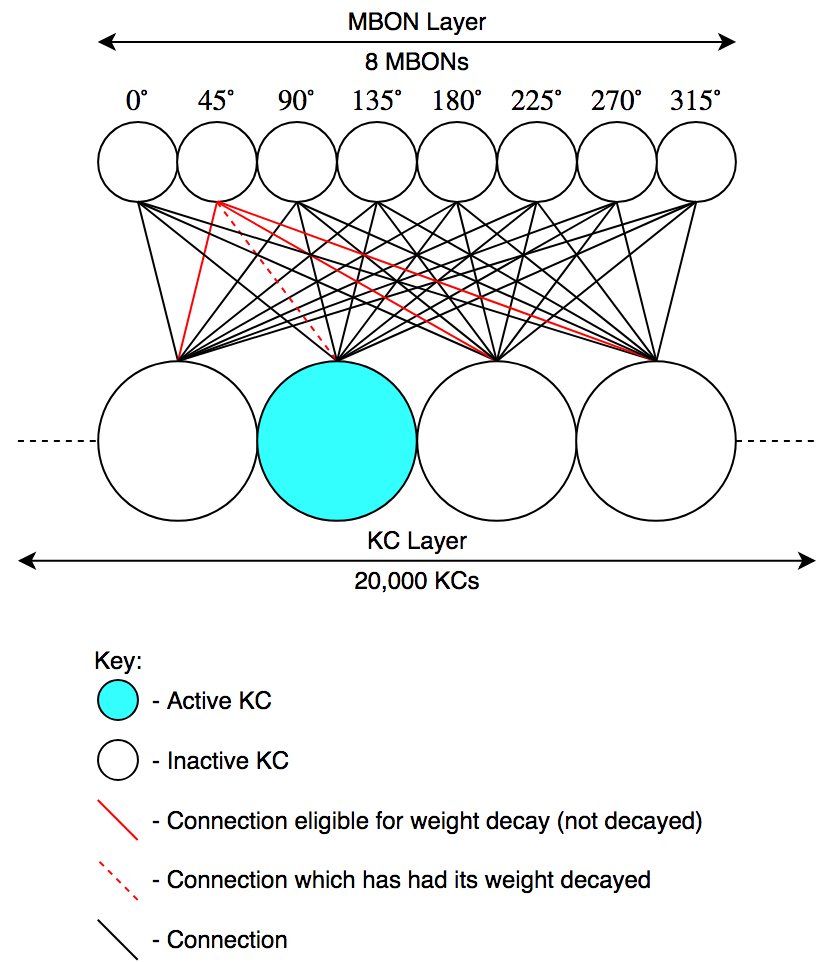
\includegraphics[width=0.9\textwidth]{EightENModel}
  \caption{\label{fig:eightmbon} Our interpretation of the eight MBON model
    proposed by \textit{Zhang}. Every KC connects to every MBON. All connection
    weights start out at $w=1$. Following the example presented in the text,
    if an image being learned corresponds to facing a direction of $45^{\circ}$,
    then only the conncetions to that MBON (highlighted in red) are eligible to
    have their weights modified. Recall, however, that these weights will only
    be modified if the KC was activated (not shown in the figure).
    }
\end{figure}


\subsection{ The Central Complex for Path Integration } \label{CXBackground}
\newpage

%%%%%%%%%%%%%%%%%%%%%%%%%%%%%%%%%%%%%%%%%%%%%%%%%%%%%%%%%%%%%%%%%%%%%%%%%%%%%%%
% PLATFORM                                                                    %
%%%%%%%%%%%%%%%%%%%%%%%%%%%%%%%%%%%%%%%%%%%%%%%%%%%%%%%%%%%%%%%%%%%%%%%%%%%%%%%
% High level description of the platform. This section can be short. Refer back
% to Part 1 for detail.
\section{ Platform } \label{sec:platform}
\subsection{ Hardware }
\subsection{ Software }
\subsubsection{ Android } \label{subsubsec:droid}
\subsubsection{ Arduino }
\subsection{ Modifications }
\newpage

%%%%%%%%%%%%%%%%%%%%%%%%%%%%%%%%%%%%%%%%%%%%%%%%%%%%%%%%%%%%%%%%%%%%%%%%%%%%%%%
% METHODS                                                                     %
%%%%%%%%%%%%%%%%%%%%%%%%%%%%%%%%%%%%%%%%%%%%%%%%%%%%%%%%%%%%%%%%%%%%%%%%%%%%%%%
\section{ Methods } \label{sec:methods}
\textit{
  Methods not final, these are included as a rough plan/guide.
  }
\subsection{ Optical Flow }
% Discuss new method (eight directional FOEs)
\subsection{ Visual Navigation }
% Discuss directional recognition, as opposed to scanning.
\subsection{ Path Integration }
% Discuss CX implementation
\subsection{ The Complete System}

\section{Experimentation}\label{sec:test}
\textit{
  Experimentation methods not final, anything in this section illustrates a
  rough plan only.
}
\subsection{General}
\subsection{Collision Avoidance}
% Write new collision avoidance system, test it independently
\subsection{Visual Navigation}
% Do the same for the MB
\subsection{Path Integration}
% And for PI
\newpage

\section{ Results and Evaluation } \label{sec:results}
\textit{Included for skeleton purposes.}
\newpage

\section{ Discussion }
\textit{Included for skeleton purposes.}
\newpage

\bibliographystyle{plain}
\bibliography{working}
\end{document}

